%##################################################################################################

\documentclass[11pt,letterpaper]{article}
%##################################################################################################

\usepackage{color}
    \definecolor{dark_blue}{rgb}{0,0,0.6}
    \definecolor{light_blue}{rgb}{0,0.4,0.8}
    \definecolor{dark_vilet}{rgb}{0.4,0,0.4}
\usepackage{fancybox}
\usepackage{wallpaper}
\usepackage{url}
\usepackage[colorlinks,
            linkcolor=dark_vilet,
            citecolor=light_blue,
            urlcolor=dark_blue]{hyperref}
\usepackage{colortbl}
\usepackage{amssymb}
\usepackage{amsmath}
\usepackage{graphicx}
\usepackage{algorithm}
\usepackage{algorithmic}
%\usepackage[square,comma,sort&compress]{natbib}
\usepackage[Sonny]{fncychap}
\usepackage{fancyhdr}
\usepackage[margin=1.5in]{geometry}
\usepackage{titletoc}
\usepackage[scaled=.92]{helvet}
\usepackage{mathptmx}
\usepackage{subfigure}
\usepackage{xspace}
\usepackage{multirow}
\usepackage[raggedright]{sidecap}

\renewcommand{\headrulewidth}{0.5pt}
\renewcommand{\footrulewidth}{0.5pt}
\ChTitleVar{\huge\sf}
\ChNameVar{\Huge\sf}
\rhead{}

\newcommand{\cdl}[1]{\textsf{#1}}
\newenvironment{link_url}
{\begin{description}
    \item}
{\end{description}}
\newenvironment{cmd_line}
{\begin{description}
    \item}
{\end{description}}

\newcommand{\ignore}[1]{}
\newcommand{\tabwidth}[0]{.45\linewidth}
\newcommand{\figwidth}[0]{.48\linewidth}

\newcommand\prjfnt{{\small \fontfamily{pag}\selectfont{}}\xspace}
\newcommand\gefnt{{\small \fontfamily{ppl}\selectfont{}}\xspace}
\newcommand{\PLASMA}{{\prjfnt{PLASMA}}\xspace}
\newcommand{\MAGMA}{{\prjfnt{MAGMA}}\xspace}
\newcommand{\TBLAS}{{\prjfnt{TBLAS}}\xspace}
\newcommand{\PBLAS}{{\prjfnt{PBLAS}}\xspace}
\newcommand{\PESSL}{{\prjfnt{PESSL}}\xspace}
\newcommand{\ESSL}{{\prjfnt{ESSL}}\xspace}
\newcommand{\SMPSS}{{\prjfnt{SMPSs}}\xspace}
\newcommand{\SMPSs}{{\prjfnt{SMPSs}}\xspace}
\newcommand{\MKL}{{\prjfnt{MKL}}\xspace}
\newcommand{\SCALAPACK}{{\prjfnt{ScaLAPACK}}\xspace}
\newcommand{\LAPACK}{{\prjfnt{LAPACK}}\xspace}
\newcommand{\LINPACK}{{\prjfnt{LINPACK}}\xspace}
\newcommand{\EISPACK}{{\prjfnt{EISPACK}}\xspace}
\newcommand{\DPOTRF}{{\gefnt{DPOTRF}}\xspace}
\newcommand{\DGEQRF}{{\gefnt{DGEQRF}}\xspace}
\newcommand{\DGETRF}{{\gefnt{DGETRF}}\xspace}
\newcommand{\DGEMM}{{\gefnt{DGEMM}}\xspace}
\newcommand{\BLAS}{{\gefnt{BLAS}}\xspace}
\newcommand{\BLACS}{{\gefnt{BLACS}}\xspace}
\newcommand{\dgemm}{{\gefnt{dgemm-seq}}\xspace}
\newcommand{\dssrfb}{{\gefnt{dssrfb-seq}}\xspace}
\newcommand{\dssssm}{{\gefnt{dssssm-seq}}\xspace}
\newcommand{\Intel}{{\gefnt{Intel64}}\xspace}
\newcommand{\Power}{{\gefnt{Power6}}\xspace}

%##################################################################################################

\begin{document}

%//////////////////////////////////////////////////////////////////////////////////////////////////

\thispagestyle{empty}
\begin{flushright}
\sf
\noindent
{\Huge\textbf{PLASMA TAU Guide}}
\rule[-1ex]{\textwidth}{5pt}\\[2.5ex]
{\Large\textbf{Parallel Linear Algebra Software for Multicore Architectures}} \\
\vspace{0.1in}
{\Large{Version 2.0}} \\
\vspace{0.5in}

\noindent
Electrical Engineering and Computer Science \\
\textbf{University of Tennessee}
\vspace{0.2in}

\noindent
Electrical Engineering and Computer Science \\
\textbf{University of California Berkeley}
\vspace{0.2in}

\noindent
Mathematical \& Statistical Sciences \\
\textbf{University of Colorado Denver}
\vspace{4.4in}

\noindent
Jack Dongarra \\
Joshua Hoffman \\
Jakub Kurzak
\end{flushright}

%//////////////////////////////////////////////////////////////////////////////////////////////////

\tableofcontents
\pagenumbering{roman}
\pagestyle{fancy}
\setlength\parindent{0in}
\setlength\parskip{0.1in}
\sloppy
\rm

%//////////////////////////////////////////////////////////////////////////////////////////////////

\newpage
\section{Introduction}
\setcounter{page}{1}
\pagenumbering{arabic}

To better understand the scheduling and inner workings of PLASMA, profiles and function traces can be used to see exactly what the PLASMA libraries are doing at any point during execution. This document will guide the reader through installing TAU (Tuning and Analysis Utilities) from the University of Oregon, and how to instrument the PLASMA libraries with the TAU tool.

%//////////////////////////////////////////////////////////////////////////////////////////////////

\section{Required Files}
Two separate downloads are required for the TAU tools. The first is the TAU tool itself, which is downloaded in a single tarball from the University of Oregon. Next, the tool used to automatically instrument the source code, called the PDT (Program Database Toolkit), can be downloaded from the same site. Finally, to view the slog2 traces, the Jumpshot-4 trace viewer is needed.

\subsection{Downloads}
All three downloads will be downloaded as tarball files, containing a root directory with their own file trees. Each package will have more detailed installation instructions included, supplementing the online documentation.

\subsubsection{TAU and PDT}
The TAU tools themselves, as well as the PDT, can both be downloaded from:
\begin{link_url}
\texttt{\url{http://www.cs.uoregon.edu/research/tau/home.php}}
\end{link_url}

Near the top left corner, click download, fill out the short information form, then download the latest version of TAU, as well as the PDT, located further down the page.

\subsubsection{slog2rte and Jumpshot-4}
It is recommended that the slog2 trace format be used when gathering traces using TAU. To generate the traces, no extra software, other than TAU and PDT, are required. However, to view the traces, the Jumpshot-4 trace viewer is required. This guide assumes the use of the slog2 format and Jumpshot-4 viewer. The Jumpshot-4 viewer can be downloaded from:
\begin{link_url}
\texttt{\url{ftp://ftp.mcs.anl.gov/pub/mpi/slog2/slog2rte.tar.gz}}
\end{link_url}

The viewer itself can be found in the folder (PATH\_TO\_SLOG2)/slog2rte/lib, and is called jumpshot.jar. A version of the java runtime environment is required to use Jumpshot. Furthermore, the Jumpshot-4 viewer can be run on any system with a graphical user interface and the java runtime environment installed.

%//////////////////////////////////////////////////////////////////////////////////////////////////

\section{Forward General Reference}
\begin{tabular}{ l }
{\it Set environment variables:} \\
{\tt \$ export PATH=/path/to/tau/x86\_64/bin:\$PATH} \\
{\tt \$ export TAU\_MAKEFILE=/path/to/tau/x86\_64/lib/Makefile.tau.pthread-pdt-trace} \\
{\it Edit your makefile and set:} {\tt cc=tau\_cc.sh; f90=tau\_f90.sh; cxx=tau\_cxx.sh} \\
{\it Compile and link with TAU, PDT:} \\
{\tt \$ make} \\
{\tt ...} \\
{\tt \$ ./your\_tau\_linked\_program.out} \\
{\tt ...} \\
{\tt \$ tau\_treemerge} \\
{\tt ...} \\
{\tt \$ tau2slog2 tau.trc tau.edf -o $<$output$>$.slog2} \\
{\tt ...} \\
{\it Using the SLOG-2 Runtime:} \\
{\tt \$ java -jar /path/to/jumpshot/jumpshot.jar} \\
\end{tabular}

%//////////////////////////////////////////////////////////////////////////////////////////////////

\section{Setup and Installation}
The tools downloaded above will need to be built on a system with access to C/C++ compilers, as well as a Java SDK and runtime environment. The required Java files can be downloaded from:
\begin{link_url}
\texttt{\url{http://java.sun.com/javase/downloads/index.jsp}}
\end{link_url}

Administrator or superuser access is not required to build or install the libraries. However, before beginning installation make sure they are in a place in where your user account has read/write/execute privileges. Also, before beginning installation, for both TAU and PDT create directories separate from their respective installation directories.

\subsection{Environment Variables}
The installation of the two packages and the Jumpshot-4 viewer require the modification of several environment variables. First, the location of the Java jvm must be located and added to the environment variable JAVA\_HOME. For example:
\begin{cmd_line}
\texttt{export JAVA\_HOME=/usr/lib/jvm/java-6-sun}
\end{cmd_line}

Next, the path to the TAU and PDT tools must be added to the path, e.g.:
\begin{cmd_line}
\texttt{export PATH=\$PATH:/home/user/pdt/x86\_64/bin:/home/user/tau/x86\_64/bin}
\end{cmd_line}

Also, for some compilers (Intel, for example) the LD\_LIBRARY\_PATH must be changed to point to the location of your compiler's libraries ((INTEL\_COMPILER\_ROOT)/lib for example). And finally, after the tools have been built and installed correctly, the TAU\_MAKEFILE environment variable will need to be created, pointing to the makefile containing the proper TAU settings. This will be discussed more at the end of the TAU installation section.

\subsection{Building PDT}
The PDT package is required for automatic instrumentation of source code to produce data with the TAU library. After downloading and extracting the PDT code, navigate to the extracted directory in the command line. The first step is to run the configure script in the top level PDT directory. The various options for the configure script are detailed in the README included with the PDT software, however three are worth noting here.

First, the configure script must be told which C++ compiler version to use via a command line option. The PDT software supports 10 compiler packages, which are listed in the README, however two of the more common ones are for the Intel package and the GNU compilers; -icpc and -GNU, respectively. The next command line options are optional, however using them will help keep everything organized. Using the -prefix=$<$dir$>$ option will allow you to specify a target directory for the installation instead of installing into the source directories. Also, the -compdir=$<$name$>$ will help keep the files organized.
An example command would look like:
\begin{cmd_line}
\texttt{./configure -icpc -prefix=/home/user/PDT -compdir=intel}
\end{cmd_line}

After the configure script has been executed, run make, then make install, and the PDT tools will be built and installed in the directory chosen above.

\subsection{Building slog2sdk}
With the slog2 run time environment, nothing new needs to be built. All of the files come as executable Java .jar files.

\subsection{Building TAU}
Configuring TAU is slightly more involved than building the PDT. Before running the configure script for TAU, make sure the environment variables above (other than TAU\_MAKEFILE for now) are set. Also, know the location of the top level PDT directory. Finally, read the INSTALL file included in the extracted TAU files to get an idea of which options best suit your needs.

The following command will configure TAU to produce slog2 traces using Intel compilers and install TAU into the directory pointed to by the -prefix=$<$directory$>$ directory. Programs will be built using the pthreads threading library as well. Programs built with the TAU compiler scripts will be automatically instrumented using the PDT built above.
\begin{cmd_line}
\texttt{./configure -pdt=/home/user/pdt -pdtcompdir=intel -cc=icc -c++=icpc
        -fortran=intel -pthread -slog2 -TRACE - PROFILE -prefix=/home/user/tau}
\end{cmd_line}

Once the script has completed, run
\begin{cmd_line}
\texttt{make install}
\end{cmd_line}
in the top level TAU directory, and upon successful completion, the TAU libraries will be built and installed under your system's architecture folder (x86\_64 for example) in the directory specified by the -prefix= option. The only thing left is to set the TAU\_MAKEFILE environment variable. From the top level TAU installation directory, change directories to the folder named after your system's architecture, and then the lib directory. In the lib directory, find the makefile which best describes the options used in the configure script(e.g. Makefile.tau-icpc-pthread-pdt-profile-trace). Now, set the environment variable TAU\_MAKEFILE to the FULL PATH to this file, including file name.

In the directory pointed to by the -prefix= option above, a folder called `examples' will have been created as well. Inside are directories containing over 50 example programs and makefiles to test the various functions of TAU. Refer to the file examples/README for a detailed description of each example.

\subsection{Instrumenting Code}
Once TAU and PDT are built and installed correctly, and the environment variables are set properly, it is a good idea to run several tests before using the tools on complicated code. In the top level of the TAU installation directory, there is an examples directory containing over 50 different programs to test the tools on. Simply change directories to one of these examples and run make to build the example. The pthreads TAU example is a good example to start with. It will pause for 5 seconds during execution, so do not panic.

To instrument your own projects with TAU, your code will need to be compiled with the compiler scripts created by TAU. For C files, the tau\_cc.sh compiler should be used, and for tau\_f90.sh for FORTRAN. For simplicity, the compiler option inside your makefiles can be changed to the necessary TAU compilers, and make can be run as usual. A simple makefile might look like:

\begin{verbatim}
CC     = tau_cc.sh
INC    = -I/home/user/intel/mkl/include
LIB    = -mkl_em64t -lguide
LIBDIR = -L/home/user/intel/mkl/lib/em64t

all:
    $(CC) $(INC) $(LIBDIR) $(LIB) test.c -o test
\end{verbatim}

Notice the makefile is a normal makefile, with just the compiler variable changed.

\subsubsection{Select File Instrumentation}
Because of the overhead associated with profiling with TAU, PLASMA performance will suffer. However, this can be avoided by only tracing important functions, reducing the performance hit caused by TAU. This can be done at compile time, by appending -optTauSelectFile=$<$path\_to\_select\_file$>$ to the TAU\_OPTIONS environment variable. The file pointed to by $<$path\_to\_select\_file$>$ is the select file PDT will use when instrumenting the program.

Select files are a powerful tool, and only a brief overview of their capabilities will be discussed here. For more information regarding select files, refer to the TAU online documentation.

The TAU select file tells PDT at compile time which functions to instrument and which ones to skip. Not only that, but it can also specify entire files to skip or include.

The select file itself is a simple text file, with any file extension; however for convenience this guide will refer to it as select.tau.

Creating a select file is fairly simple; it consists of lists of files or functions to include or exclude and the flags to mark the beginning or end of a list. To include or exclude files, the lists are surrounded by:
BEGIN\_FILE\_INCLUDE\_LIST / END\_FILE\_INCLUDE\_LIST and
BEGIN\_FILE\_EXCLUDE\_LIST / END\_FILE\_EXCLUDE\_LIST markers respectively.

To make selecting file easier, TAU supports the use of two wildcards (* and ?) in file include/exclude lists. The first, *, matches any number of characters while ? only matches one. Also, \# can be used for comment lines. An example section of a select file which has an exclude file list would look like:

\begin{verbatim}
BEGIN_FILE_EXCLUDE_LIST

# exclude all files with a .f extension
*.f

# exclude files beginning with main.
# with a single letter file extension
main.?

END_FILE_EXCLUDE_LIST
\end{verbatim}

Similarly, the function include/exclude lists are encased by
BEGIN\_INCLUDE\_LIST / END\_INCLUDE\_LIST and BEGIN\_EXCLUDE\_LIST / END\_EXCLUDE\_LIST markers, respectively. The function include/exclude lists are slightly more difficult than the file lists because the functions must have an argument type list as well as a return type. Also, if using mixed FORTRAN and C code as in PLASMA, a capital letter `C' is required at the end of each function listing in the select file. Unlike the file lists above, the function lists only have one wildcard symbol `\#'. However, the wildcard only matches against function names; a correct argument list and return type are still required. If used at the beginning of the line, `\#' will still mark a commented line.
For example, the following is a snippet from a select file excluding several functions.

\begin{verbatim}
BEGIN_EXCLUDE_LIST

double get_current_time(void) C

# the next line excludes all functions beginning with sort_
# which return void and accept int *
void sort_#(int *) C

# FORTRAN subroutines only require the name of the subroutine
CORE_DGESSM

END_EXCLUDE_LIST
\end{verbatim}

Select file instrumentation also supports an instrument section, where specific functions may be instrumented differently, as well as tracking different memory allocations/deallocations and loop specific instrumentation. However, these are beyond the scope of this document; please refer to the TAU documentation for more information about select file instrument sections.

\subsubsection{Compiling PLASMA with TAU}
To compile plasma with TAU, make sure the make.inc.example file is correctly renamed `make.inc'. Then, edit the make.inc file so that the lines

\begin{verbatim}
CC     = icc
FC     = ifort
LINKER = ifort
\end{verbatim}

are changed to

\begin{verbatim}
CC     = tau_cc.sh
FC     = tau_f90.sh
LINKER = tau_f90.sh
\end{verbatim}

Also, ensure that the INC, LIB, and LIBDIR variables correspond to your BLAS. Then, run make as usual. If the build is successful, test PLASMA and TAU using the files included in the `testing' directory.

%//////////////////////////////////////////////////////////////////////////////////////////////////

\section{Using TAU}
After the executables have been built using the TAU compilers and are properly instrumented, all that remains is to run the code on a sufficiently large data set, to gain a clear picture of what the code is doing; for PLASMA code a matrix of at least 1000x1000 is recommended.

To localize profile and trace output from TAU, two environment variables can be set to point to a directory where the corresponding output will be dumped. It is recommended to set a different output location for each program run, and for runs you wish to keep separated; TAU output files will overwrite previous data. The two environment variables are \mbox{PROFILEDIR} and \mbox{TRACEDIR}. Set these to their target directories, and TAU will automatically put the output files here at run time.

\subsection{Trace Format Conversion}
Once the code is finished executing, several files will be created in the current directory. These files are events.0.edf, and tautrace.0.0.*.trc, where * is a specific processor number. Each processor core used will have it's own file created. Before these files can be converted to slog2 format, they first must be merged into a single file. This is simply done by running {\tt tau\_treemerge} from the command line (assuming the PATH is set properly) in the directory in which the files are located. This creates two new  files, tau.edf and tau.trc.
The next step is to convert these two new files into slog2 format. Just run {\tt tau2slog2 tau.trc tau.edf -o $<$output$>$.slog2} from the command line, where $<$output$>$ is the desired name of the trace file.

\subsection{Viewing slog2 Trace}
With the TAU trace converted to slog2 format, open the Jumpshot viewer by executing the Java .jar file, jumpshot.jar. Click the ``Select new logfile'' button in the bottom left hand corner of the viewer (Figure~\ref{fig:select_button}), then navigate to the .slog2 file output by tau2slog2, click it, and then select open in the dialog box. After choosing and opening the .slog2 file, three windows should appear
(Figure~\ref{fig:three_windows}).

\begin{figure}
\centering
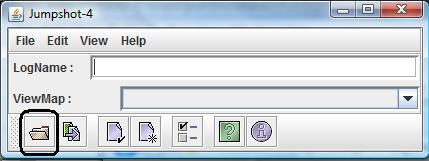
\includegraphics[scale=0.8]{step0.jpg}
\caption{Button to open file select dialog.}
\label{fig:select_button}
\end{figure}

\begin{figure}
\centering
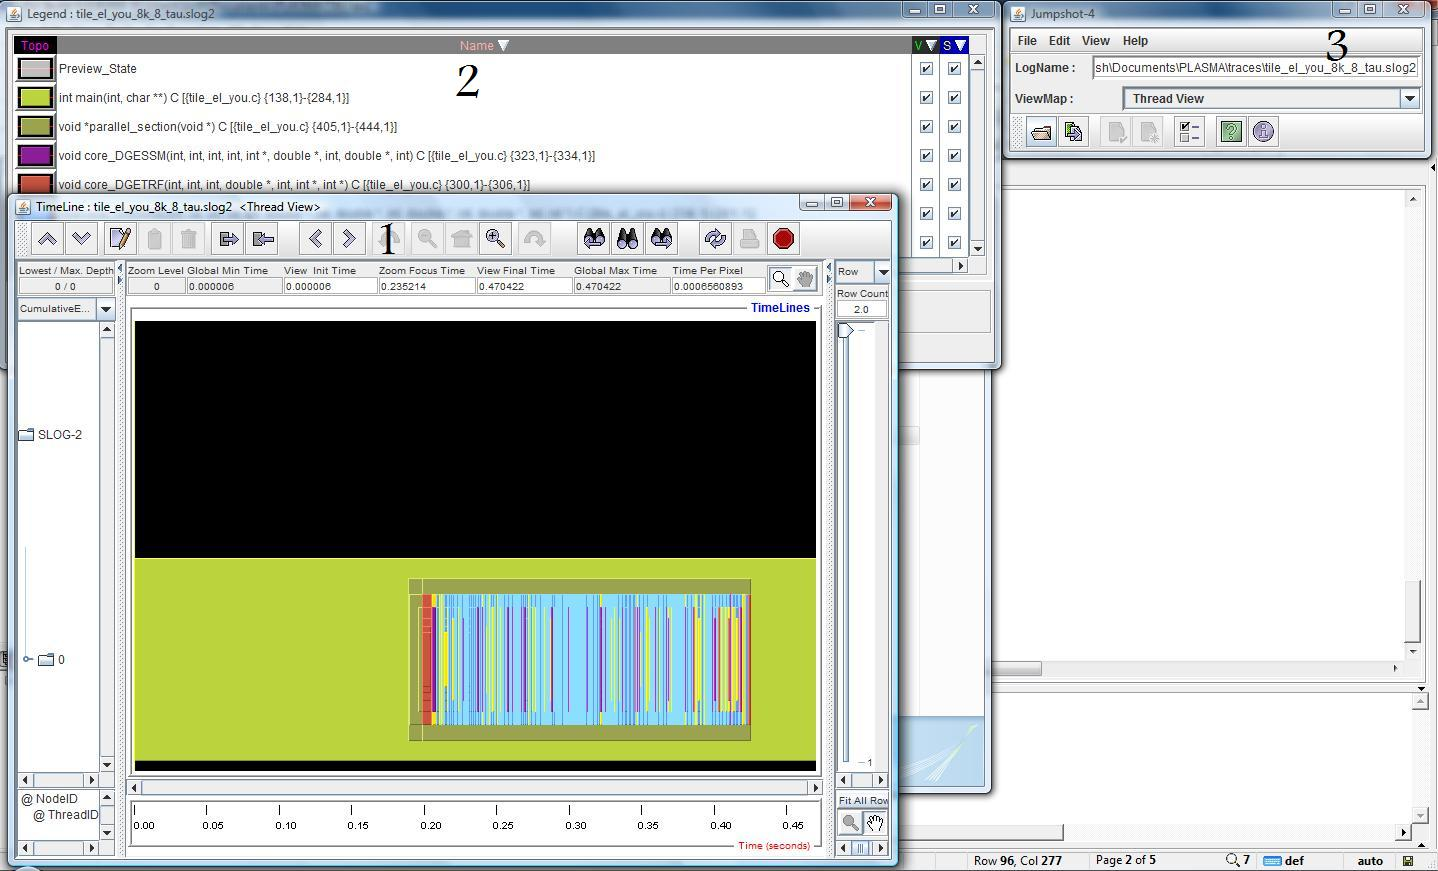
\includegraphics[scale=0.32]{step1.jpg}
\caption{Trace window (1), legend window(2), and viewer window (3).}
\label{fig:three_windows}
\end{figure}

Window 1 is where the trace will be displayed. Window 2 is the legend, where the colors of the trace window are related to the functions traced in the program. Window 3 is the Jumpshot viewer window, where a new file can be opened and Jumpshot options modified.

To view the function trace for each thread, find the ``ViewMap'' drop-down box on the Jumpshot-4 viewer, then select Identity Map. This changes the trace window to show the activity of each thread. The trace window should change to look like the one on Figure~\ref{fig:trace_window}.

\begin{figure}
\centering
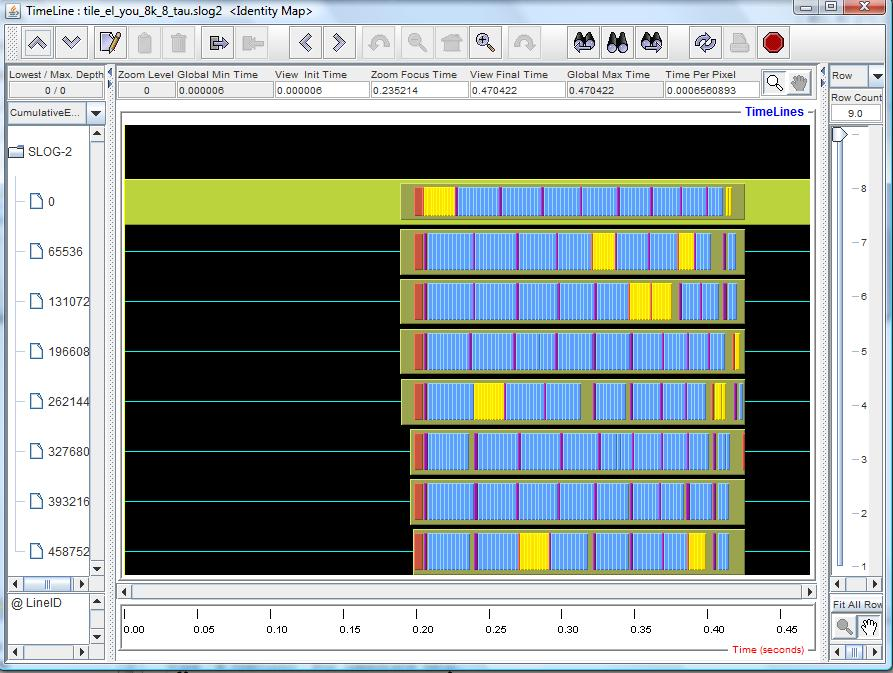
\includegraphics[scale=0.5]{step2.jpg}
\caption{Trace view window after Identity Map has been selected.}
\label{fig:trace_window}
\end{figure}

Depending on your program, this view might contain a large amount of information that can be difficult to interpret. However, using the legend, extraneous functions can be removed to give a clearer view of the important information. First, with the legend window active, uncheck boxes in the `V' column that correspond to functions to be removed (Figure~\ref{fig:checkboxes}).

\begin{figure}
\centering
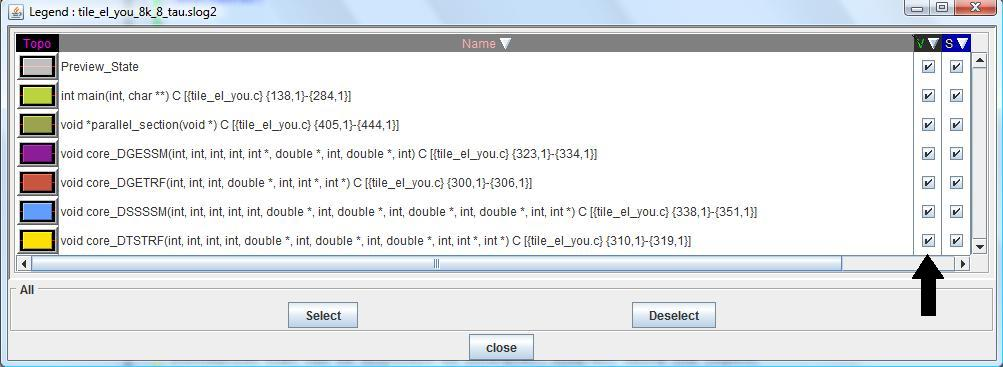
\includegraphics[scale=0.45]{step3.jpg}
\caption{The legend window. The arrow points to the checkboxes which can be used to turn on and off
         displaying of individual functions.}
\label{fig:checkboxes}
\end{figure}

After unchecking the boxes in the legend window, the trace will still look the same. At the top of the trace window, click the 
\includegraphics{step4.jpg} button to refresh the trace. The trace window should now resemble the two traces in the following examples section.

To produce a trace showing the work PLASMA is doing, only the functions and files in the (PLASMA\_DIR)/core\_blas folder need to be traced.

%//////////////////////////////////////////////////////////////////////////////////////////////////

\section{Examples}
Figures~\ref{fig:plasma_8} and \ref{fig:plasma_16} show what a trace of PLASMA should look like. Both traces only include the functions found in the (PLASMA\_DIR)/core\_blas directory, the main function and the parallel\_section function.

\begin{figure}
\centering
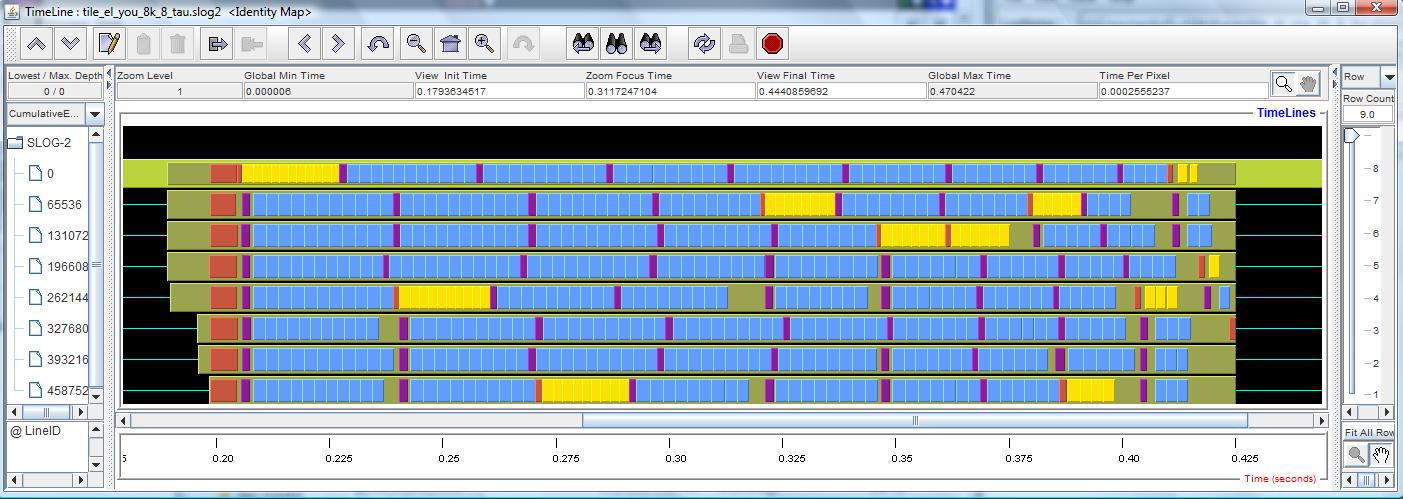
\includegraphics[scale=0.32]{tile_el_you_8k_tau.jpg}
\caption{Sample TAU trace of PLASMA tile LU factorization on 8 cores.}
\label{fig:plasma_8}
\end{figure}

\begin{figure}
\centering
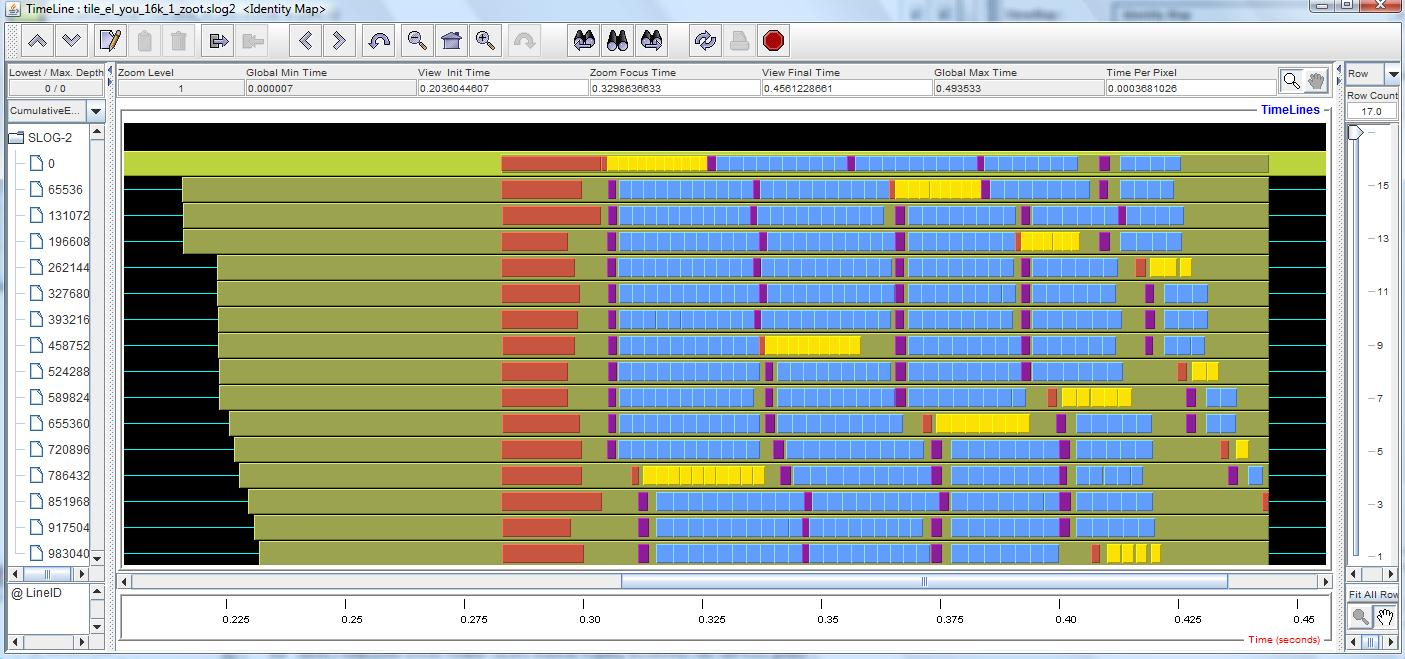
\includegraphics[scale=0.32]{tile_el_you_16k_tau.jpg}
\caption{Sample TAU trace of PLASMA tile LU factorization on 16 cores.}
\label{fig:plasma_16}
\end{figure}

%##################################################################################################

\end{document}
